\subsubsection{Web Site}
\paragraph*{Events}
In order to better understand the remote client web site, it is necessary to identify the events that may occur, which are presented in table \ref{table:rc_web_events}.

\begin{table}[ht]
	\centering
	\resizebox{\columnwidth}{!}
	{
		\begin{tabular}{|m{3cm}|m{5cm}|m{2.4cm}|m{2.4cm}|}
			\hline
			\textbf{Event} & \textbf{System Response} & \textbf{Source} & \textbf{Type}\\
			\hline\hline
			Insert location	& Show parking spots & User & Asynchronous\\
			\hline
			
			Obtain geolocation & Request device geolocation & Mobile Device & Asynchronous\\
			\hline
			
		\end{tabular}
	}
	\caption{Events: Remote Client Web Site.}
	\label{table:rc_web_events}
\end{table}

\paragraph*{Use Cases}
The web site use cases are shown in figure \ref{fig:UseCases_WebSite}. The main actors are the user, the remote server and a mobile device. In order to know if there are available parking spaces in a certain location, the user can enter a location (inserting the street name, for example) or, as in the mobile application, use his mobile device to obtain the location automatically. The remote server lets the user know where there are empty parking spaces.

\begin{figure}[H]
	\centering
	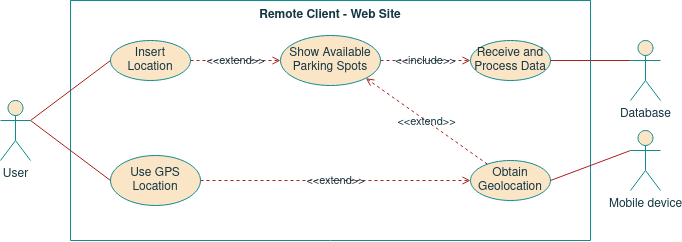
\includegraphics[width=1\textwidth]{06remote_system/WebSite_UseCases}
	\caption{Use Cases: Remote Client Web Site.}
	\label{fig:UseCases_WebSite}
\end{figure}

\clearpage
\paragraph*{State Chart}
In figure \ref{fig:StateChart_WebSite}, one can see the web site state chart. The system initiates with the system configuration. Then the user can use his mobile phone's location (through the GPS tracking system) or type manually the location address. If the user enters a location manually (the street name, for example), it will be checked and, if valid, the available parking spaces will be displayed.

\begin{figure}[H]
	\centering
	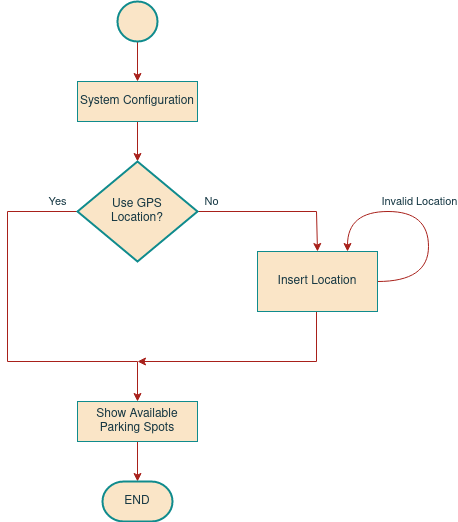
\includegraphics[width=0.8\textwidth]{06remote_system/WebSite_StateChart}
	\caption{State Chart: Remote Client Web Site.}
	\label{fig:StateChart_WebSite}
\end{figure}

\clearpage

\paragraph*{Sequence Diagram}
The sequence diagram of the web site is shown in the figure \ref{fig:SeqDiagram_WebSite}. To know where there are empty parking spots, the user can insert manually a location or use his \ac{gps} location. In both cases the web site asks the remote server if there are available parking spots near the location and displays them to the user. However, in the case of using the \ac{gps} location, the web site has to get the \ac{gps} coordinates from the mobile device running the web site.

\begin{figure}[H]
	\centering
	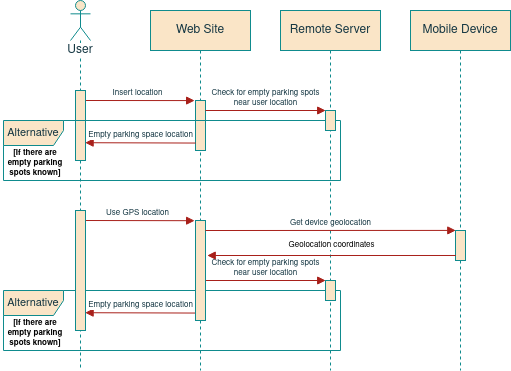
\includegraphics[width=1\textwidth]{06remote_system/WebSite_SeqDiagram}
	\caption{Sequence Diagram: Remote Client Web Site.}
	\label{fig:SeqDiagram_WebSite}
\end{figure}